% Options for packages loaded elsewhere
\PassOptionsToPackage{unicode}{hyperref}
\PassOptionsToPackage{hyphens}{url}
%
\documentclass[
  ignorenonframetext,
]{beamer}
\usepackage{pgfpages}
\setbeamertemplate{caption}[numbered]
\setbeamertemplate{caption label separator}{: }
\setbeamercolor{caption name}{fg=normal text.fg}
\beamertemplatenavigationsymbolsempty
% Prevent slide breaks in the middle of a paragraph
\widowpenalties 1 10000
\raggedbottom
\setbeamertemplate{part page}{
  \centering
  \begin{beamercolorbox}[sep=16pt,center]{part title}
    \usebeamerfont{part title}\insertpart\par
  \end{beamercolorbox}
}
\setbeamertemplate{section page}{
  \centering
  \begin{beamercolorbox}[sep=12pt,center]{part title}
    \usebeamerfont{section title}\insertsection\par
  \end{beamercolorbox}
}
\setbeamertemplate{subsection page}{
  \centering
  \begin{beamercolorbox}[sep=8pt,center]{part title}
    \usebeamerfont{subsection title}\insertsubsection\par
  \end{beamercolorbox}
}
\AtBeginPart{
  \frame{\partpage}
}
\AtBeginSection{
  \ifbibliography
  \else
    \frame{\sectionpage}
  \fi
}
\AtBeginSubsection{
  \frame{\subsectionpage}
}

\usepackage{amsmath,amssymb}
\usepackage{lmodern}
\usepackage{iftex}
\ifPDFTeX
  \usepackage[T1]{fontenc}
  \usepackage[utf8]{inputenc}
  \usepackage{textcomp} % provide euro and other symbols
\else % if luatex or xetex
  \usepackage{unicode-math}
  \defaultfontfeatures{Scale=MatchLowercase}
  \defaultfontfeatures[\rmfamily]{Ligatures=TeX,Scale=1}
\fi
\usetheme[]{defaulttheme.scss}
% Use upquote if available, for straight quotes in verbatim environments
\IfFileExists{upquote.sty}{\usepackage{upquote}}{}
\IfFileExists{microtype.sty}{% use microtype if available
  \usepackage[]{microtype}
  \UseMicrotypeSet[protrusion]{basicmath} % disable protrusion for tt fonts
}{}
\makeatletter
\@ifundefined{KOMAClassName}{% if non-KOMA class
  \IfFileExists{parskip.sty}{%
    \usepackage{parskip}
  }{% else
    \setlength{\parindent}{0pt}
    \setlength{\parskip}{6pt plus 2pt minus 1pt}}
}{% if KOMA class
  \KOMAoptions{parskip=half}}
\makeatother
\usepackage{xcolor}
\newif\ifbibliography
\setlength{\emergencystretch}{3em} % prevent overfull lines
\setcounter{secnumdepth}{-\maxdimen} % remove section numbering


\providecommand{\tightlist}{%
  \setlength{\itemsep}{0pt}\setlength{\parskip}{0pt}}\usepackage{longtable,booktabs,array}
\usepackage{calc} % for calculating minipage widths
\usepackage{caption}
% Make caption package work with longtable
\makeatletter
\def\fnum@table{\tablename~\thetable}
\makeatother
\usepackage{graphicx}
\makeatletter
\def\maxwidth{\ifdim\Gin@nat@width>\linewidth\linewidth\else\Gin@nat@width\fi}
\def\maxheight{\ifdim\Gin@nat@height>\textheight\textheight\else\Gin@nat@height\fi}
\makeatother
% Scale images if necessary, so that they will not overflow the page
% margins by default, and it is still possible to overwrite the defaults
% using explicit options in \includegraphics[width, height, ...]{}
\setkeys{Gin}{width=\maxwidth,height=\maxheight,keepaspectratio}
% Set default figure placement to htbp
\makeatletter
\def\fps@figure{htbp}
\makeatother

\makeatletter
\makeatother
\makeatletter
\makeatother
\makeatletter
\@ifpackageloaded{caption}{}{\usepackage{caption}}
\AtBeginDocument{%
\ifdefined\contentsname
  \renewcommand*\contentsname{Table of contents}
\else
  \newcommand\contentsname{Table of contents}
\fi
\ifdefined\listfigurename
  \renewcommand*\listfigurename{List of Figures}
\else
  \newcommand\listfigurename{List of Figures}
\fi
\ifdefined\listtablename
  \renewcommand*\listtablename{List of Tables}
\else
  \newcommand\listtablename{List of Tables}
\fi
\ifdefined\figurename
  \renewcommand*\figurename{Figure}
\else
  \newcommand\figurename{Figure}
\fi
\ifdefined\tablename
  \renewcommand*\tablename{Table}
\else
  \newcommand\tablename{Table}
\fi
}
\@ifpackageloaded{float}{}{\usepackage{float}}
\floatstyle{ruled}
\@ifundefined{c@chapter}{\newfloat{codelisting}{h}{lop}}{\newfloat{codelisting}{h}{lop}[chapter]}
\floatname{codelisting}{Listing}
\newcommand*\listoflistings{\listof{codelisting}{List of Listings}}
\makeatother
\makeatletter
\@ifpackageloaded{caption}{}{\usepackage{caption}}
\@ifpackageloaded{subcaption}{}{\usepackage{subcaption}}
\makeatother
\makeatletter
\@ifpackageloaded{tcolorbox}{}{\usepackage[many]{tcolorbox}}
\makeatother
\makeatletter
\@ifundefined{shadecolor}{\definecolor{shadecolor}{rgb}{.97, .97, .97}}
\makeatother
\makeatletter
\makeatother
\ifLuaTeX
  \usepackage{selnolig}  % disable illegal ligatures
\fi
\IfFileExists{bookmark.sty}{\usepackage{bookmark}}{\usepackage{hyperref}}
\IfFileExists{xurl.sty}{\usepackage{xurl}}{} % add URL line breaks if available
\urlstyle{same} % disable monospaced font for URLs
\hypersetup{
  pdftitle={Studying a concept in disarray: Cross-cultural, comparative analysis of digital privacy},
  pdfauthor={Dmitry Epstein \& Philipp K. Masur},
  hidelinks,
  pdfcreator={LaTeX via pandoc}}

\title{Studying a concept in disarray: Cross-cultural, comparative
analysis of digital privacy}
\subtitle{Minerva-Gentner Symposium 2022 in Jerusalem}
\author{Dmitry Epstein \& Philipp K. Masur}
\date{}
\logo{\includegraphics{https://comparativeprivacy.org/wp-content/uploads/2020/04/cropped-cprn\_logo.png}}

\begin{document}
\frame{\titlepage}
\ifdefined\Shaded\renewenvironment{Shaded}{\begin{tcolorbox}[breakable, borderline west={3pt}{0pt}{shadecolor}, enhanced, sharp corners, interior hidden, boxrule=0pt, frame hidden]}{\end{tcolorbox}}\fi

\hypertarget{welcome-to-jerusalem}{%
\section{WELCOME TO JERUSALEM!}\label{welcome-to-jerusalem}}

\begin{frame}{Who are we?}
\protect\hypertarget{who-are-we}{}
\begin{column}{0.45\textwidth}
\includegraphics{https://comparativeprivacy.org/wp-content/uploads/2020/04/cropped-cprn_logo.png}

\url{https://www.comparativeprivacy.org}
\end{column}

\begin{column}{0.05\textwidth}
\end{column}

\begin{column}{0.45\textwidth}
\begin{block}{Goals and Aims}
\protect\hypertarget{goals-and-aims}{}
\begin{enumerate}
\tightlist
\item
  Research Infrastructure for comparative privacy research
\item
  Guidance, learning opportunities (e.g., workshops, preconferences)
\item
  Conducting comparative privacy research in line with our proposed
  framework
\item
  Long-term: Larger continuous longitudinal survey study (akin to the
  World Value Survey)
\end{enumerate}
\end{block}
\end{column}
\end{frame}

\begin{frame}{Overview of the Symposium}
\protect\hypertarget{overview-of-the-symposium}{}
\begin{longtable}[]{@{}
  >{\raggedright\arraybackslash}p{(\columnwidth - 4\tabcolsep) * \real{0.1000}}
  >{\raggedright\arraybackslash}p{(\columnwidth - 4\tabcolsep) * \real{0.1000}}
  >{\raggedright\arraybackslash}p{(\columnwidth - 4\tabcolsep) * \real{0.8000}}@{}}
\caption{Day 1}\tabularnewline
\toprule()
\begin{minipage}[b]{\linewidth}\raggedright
Date
\end{minipage} & \begin{minipage}[b]{\linewidth}\raggedright
Time
\end{minipage} & \begin{minipage}[b]{\linewidth}\raggedright
Program
\end{minipage} \\
\midrule()
\endfirsthead
\toprule()
\begin{minipage}[b]{\linewidth}\raggedright
Date
\end{minipage} & \begin{minipage}[b]{\linewidth}\raggedright
Time
\end{minipage} & \begin{minipage}[b]{\linewidth}\raggedright
Program
\end{minipage} \\
\midrule()
\endhead
25.10. & 19:00 & Get-Together / Dinner \\
26.10. & 08:30 & Coffee and Pastries \\
& 09:00 & Setting the day: The challenge of studying privacy \\
& 09:30 & Session I: Privacy across national borders \\
& 10:45 & Coffee Break \\
& 11:00 & Session II: Comparative cases \\
& 12:15 & Lunch Break \\
& 13:30 & Keynote: Tanya Lokot \\
& 14:30 & Coffee Break \\
& 14:45 & Workshop - Part A \\
& 16:00 & Coffee Break \\
& 16:15 & Workshop - Part B \\
& 17:30 & Day Summary \\
\bottomrule()
\end{longtable}
\end{frame}

\begin{frame}{Overview of the Symposium}
\protect\hypertarget{overview-of-the-symposium-1}{}
\begin{longtable}[]{@{}
  >{\raggedright\arraybackslash}p{(\columnwidth - 4\tabcolsep) * \real{0.1000}}
  >{\raggedright\arraybackslash}p{(\columnwidth - 4\tabcolsep) * \real{0.1000}}
  >{\raggedright\arraybackslash}p{(\columnwidth - 4\tabcolsep) * \real{0.8000}}@{}}
\caption{Day 2}\tabularnewline
\toprule()
\begin{minipage}[b]{\linewidth}\raggedright
Date
\end{minipage} & \begin{minipage}[b]{\linewidth}\raggedright
Time
\end{minipage} & \begin{minipage}[b]{\linewidth}\raggedright
Program
\end{minipage} \\
\midrule()
\endfirsthead
\toprule()
\begin{minipage}[b]{\linewidth}\raggedright
Date
\end{minipage} & \begin{minipage}[b]{\linewidth}\raggedright
Time
\end{minipage} & \begin{minipage}[b]{\linewidth}\raggedright
Program
\end{minipage} \\
\midrule()
\endhead
27.10. & 08:30 & Coffee and Pastries \\
& 09:00 & Setting the day: An agenda for comparative privacy research \\
& 09:30 & Session I: New approaches to comparative privacy research \\
& 10:45 & Coffee Break \\
& 11:00 & Session II: Most burning research questions in the coming
years? \\
& 12:15 & Lunch Break \\
& 13:30 & Keynote: Tehilla Shwartz Altschuller \\
& 14:30 & Coffee Break \\
& 14:45 & Workshop - Part C \\
& 16:00 & Coffee Break \\
& 14:45 & Workshop - Part D \\
& 17:30 & Day Summary \& Goodbyes \\
\bottomrule()
\end{longtable}
\end{frame}

\begin{frame}{Thank you!}
\protect\hypertarget{thank-you}{}
\begin{itemize}
\item
  Minverva-Gentner Foundation for Israeli-German Science Exchange
\item
  Federmann Cyber Security Research Center -- Cyber Law Program
\end{itemize}
\end{frame}

\begin{frame}{What do you think?}
\protect\hypertarget{what-do-you-think}{}
\end{frame}

\begin{frame}{Privacy concerns}
\protect\hypertarget{privacy-concerns}{}
\end{frame}

\begin{frame}{Privacy concerns}
\protect\hypertarget{privacy-concerns-1}{}
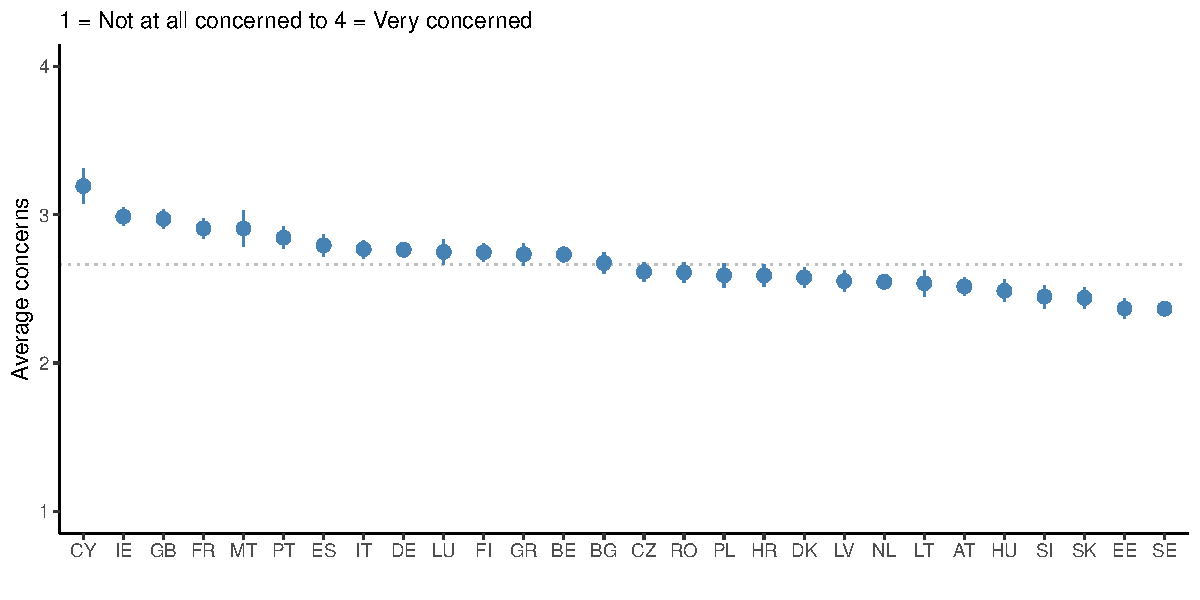
\includegraphics{slides_files/figure-beamer/unnamed-chunk-2-1.pdf}
\end{frame}

\begin{frame}{Privacy concerns}
\protect\hypertarget{privacy-concerns-2}{}
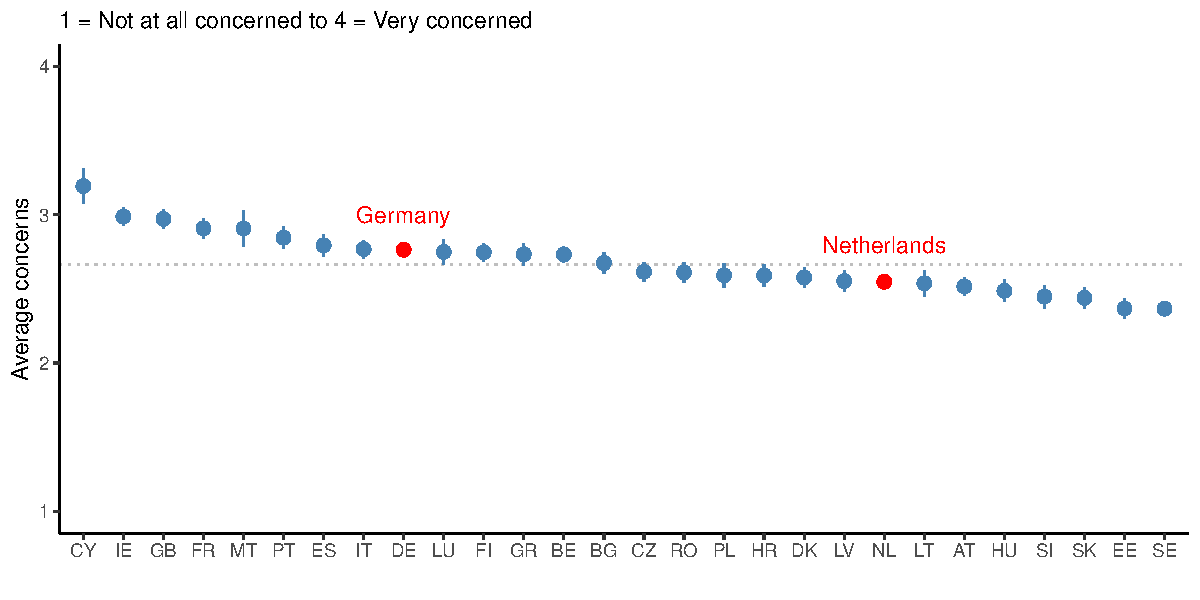
\includegraphics{slides_files/figure-beamer/unnamed-chunk-3-1.pdf}
\end{frame}

\begin{frame}{Reading privacy policies}
\protect\hypertarget{reading-privacy-policies}{}
\end{frame}

\begin{frame}{Reading privacy policies}
\protect\hypertarget{reading-privacy-policies-1}{}
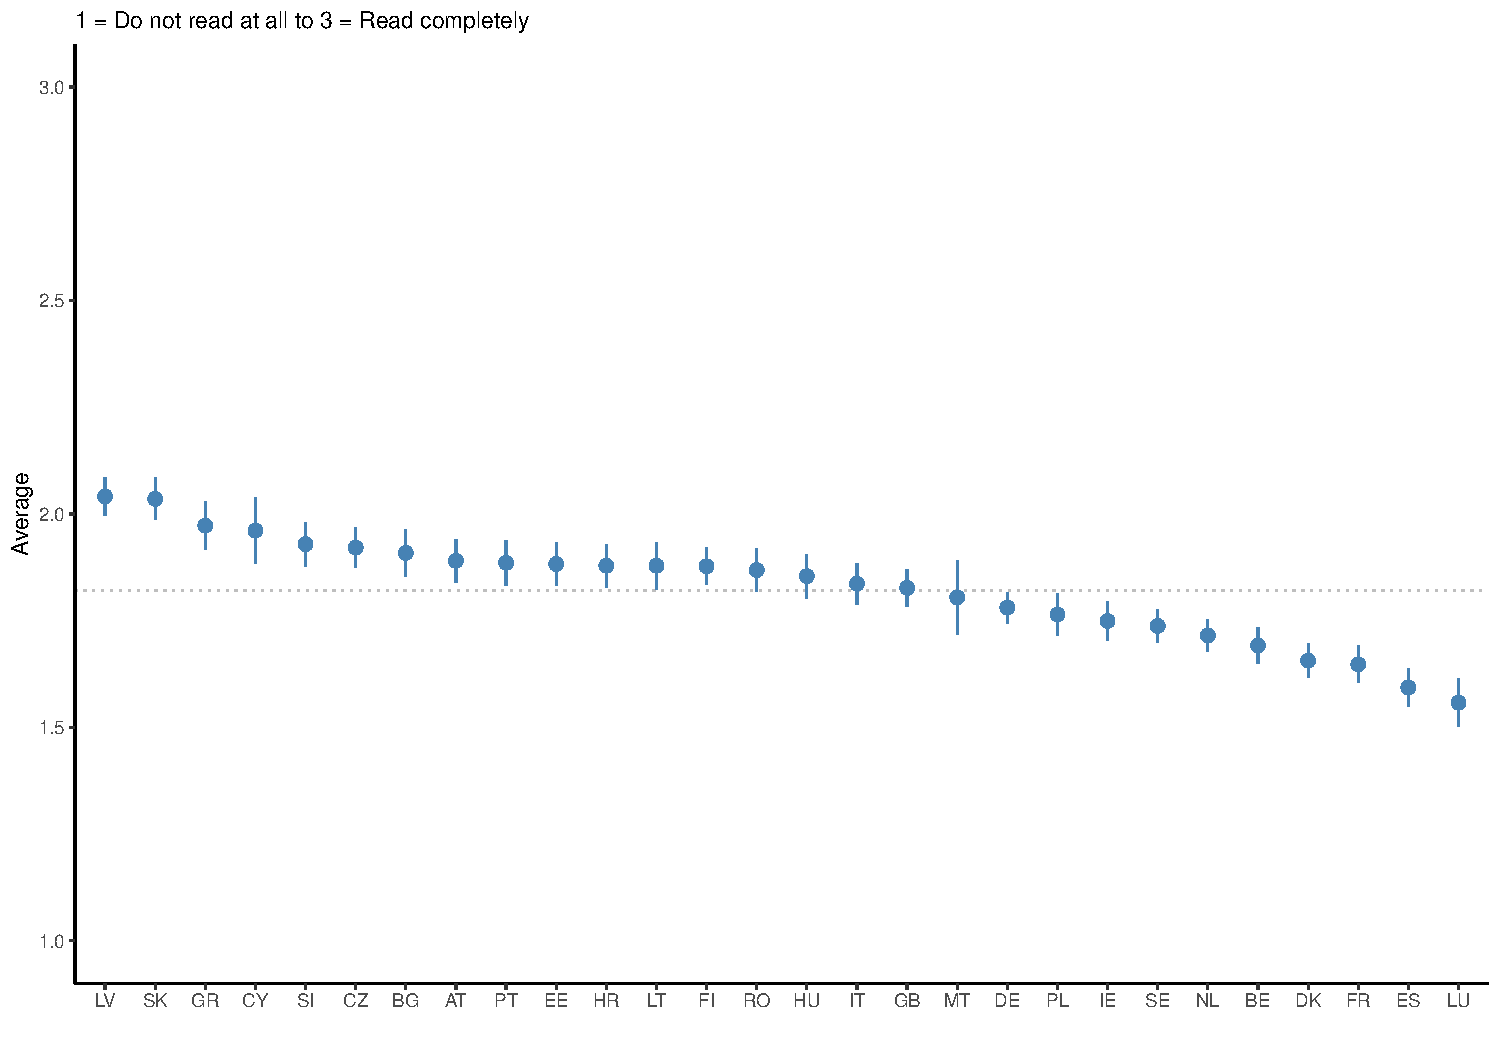
\includegraphics{slides_files/figure-beamer/unnamed-chunk-4-1.pdf}
\end{frame}

\begin{frame}{Reading privacy policies}
\protect\hypertarget{reading-privacy-policies-2}{}
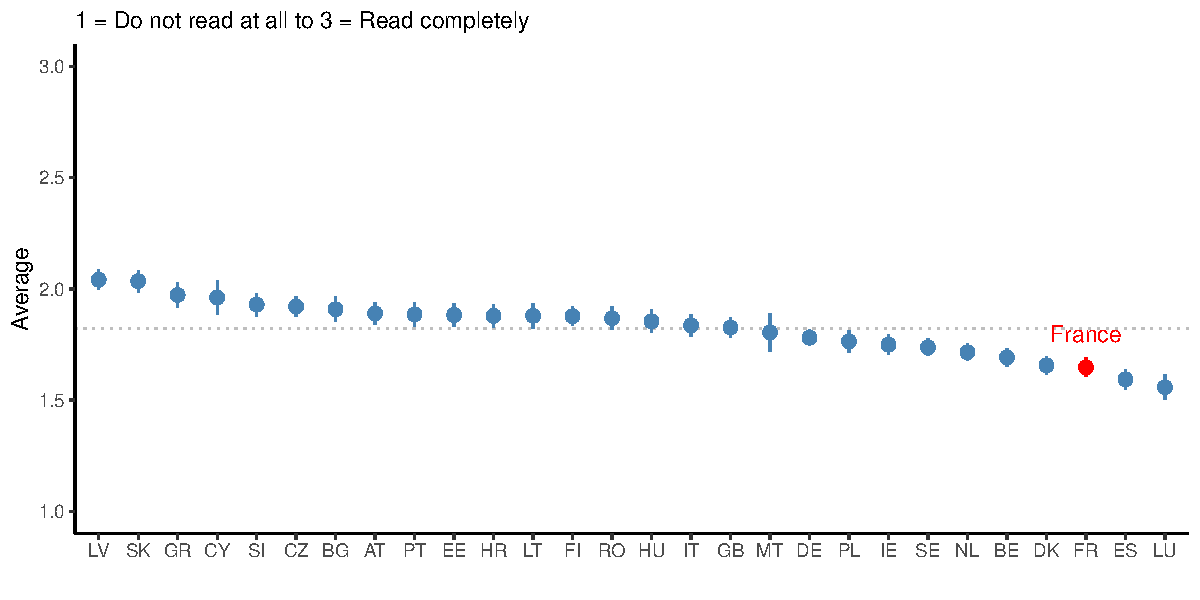
\includegraphics{slides_files/figure-beamer/unnamed-chunk-5-1.pdf}
\end{frame}

\begin{frame}{Cultures}
\protect\hypertarget{cultures}{}
\includegraphics{https://licensewithmosaiq.com/wp-content/uploads/2019/06/shutterstock_1303850926-1024x432.jpg}
\end{frame}

\begin{frame}{Political Systems}
\protect\hypertarget{political-systems}{}
\includegraphics{https://futuristspeaker.com/wp-content/uploads/2022/04/futurist-thomas-frey-democracy-vs-autocracy-what-does-the-future-hold.jpg}
\end{frame}

\begin{frame}{Technological structures}
\protect\hypertarget{technological-structures}{}
\includegraphics{https://cdn.searchenginejournal.com/wp-content/uploads/2021/09/16-reasons-why-social-media-is-important-to-your-company-616d3200e6dc6-sej.png}
\end{frame}

\begin{frame}{Much more to take into account}
\protect\hypertarget{much-more-to-take-into-account}{}
\begin{itemize}
\item
  Economies
\item
  Social disparities
\item
  Power imbalances
\item
  Socio-Demographic differences
\item
  \ldots{}
\end{itemize}
\end{frame}

\begin{frame}{Comparative Privacy Research Framework}
\protect\hypertarget{comparative-privacy-research-framework}{}
Two important questions:

\begin{enumerate}
\item
  What is the variable of interest?
\item
  What are meaningful units of comparison
\end{enumerate}
\end{frame}

\begin{frame}{Goals}
\protect\hypertarget{goals}{}
\begin{itemize}
\item
  Identifying meaningful units of comparison
\item
  Disentangling how these structures interact with privacy processes at
  micro, meso- and macro-levels
\item
  Providing a framework and agenda for systematic comparative privacy
  research
\end{itemize}
\end{frame}

\begin{frame}{Potential units of comparison}
\protect\hypertarget{potential-units-of-comparison}{}
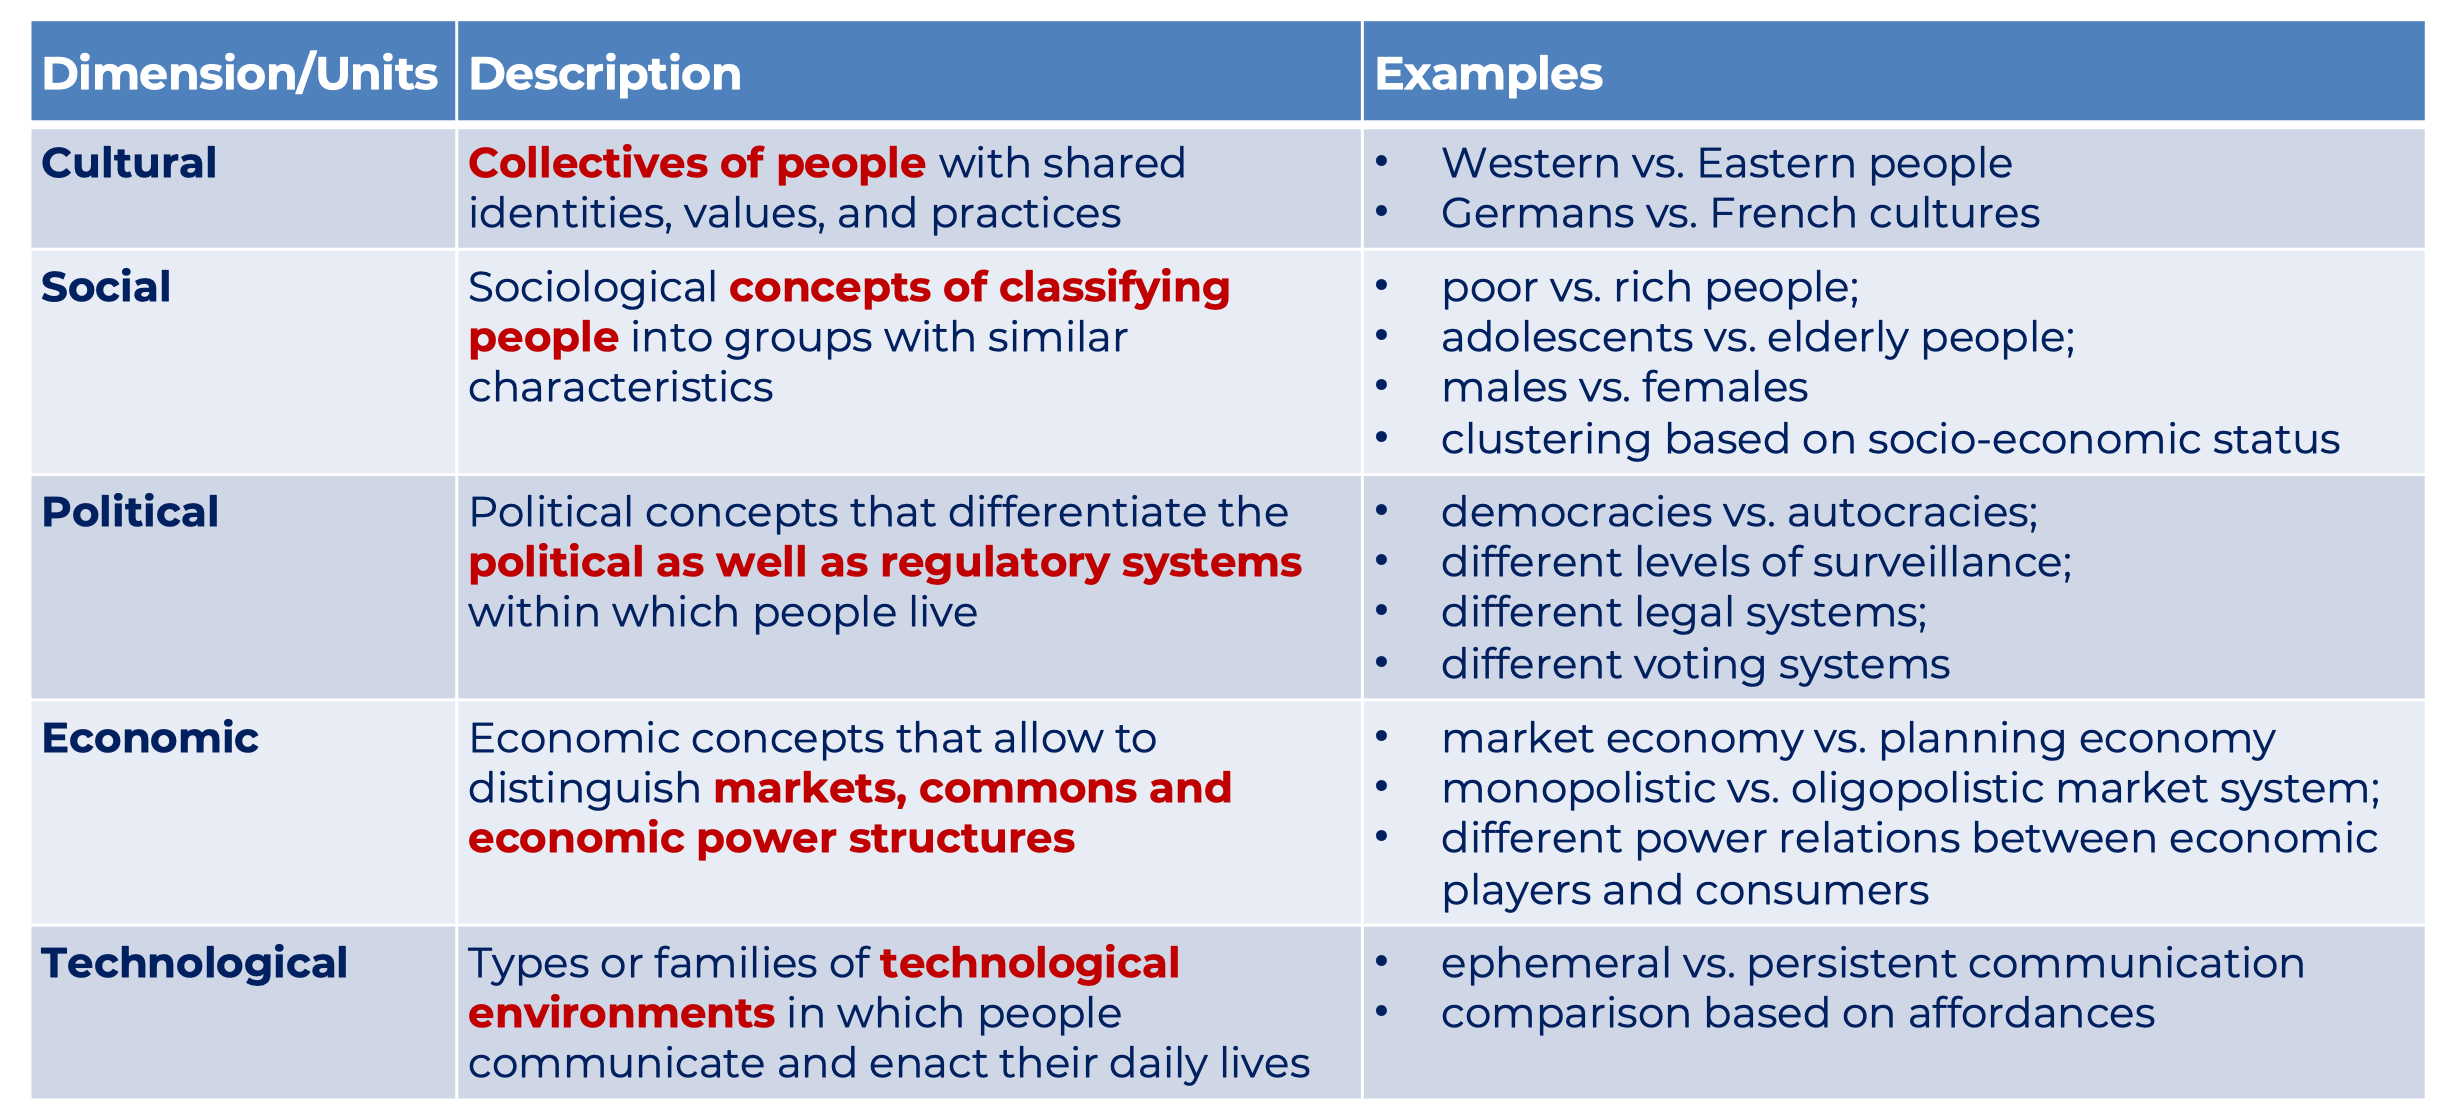
\includegraphics{img/units.png}
\end{frame}

\begin{frame}{Comparative perspectives}
\protect\hypertarget{comparative-perspectives}{}
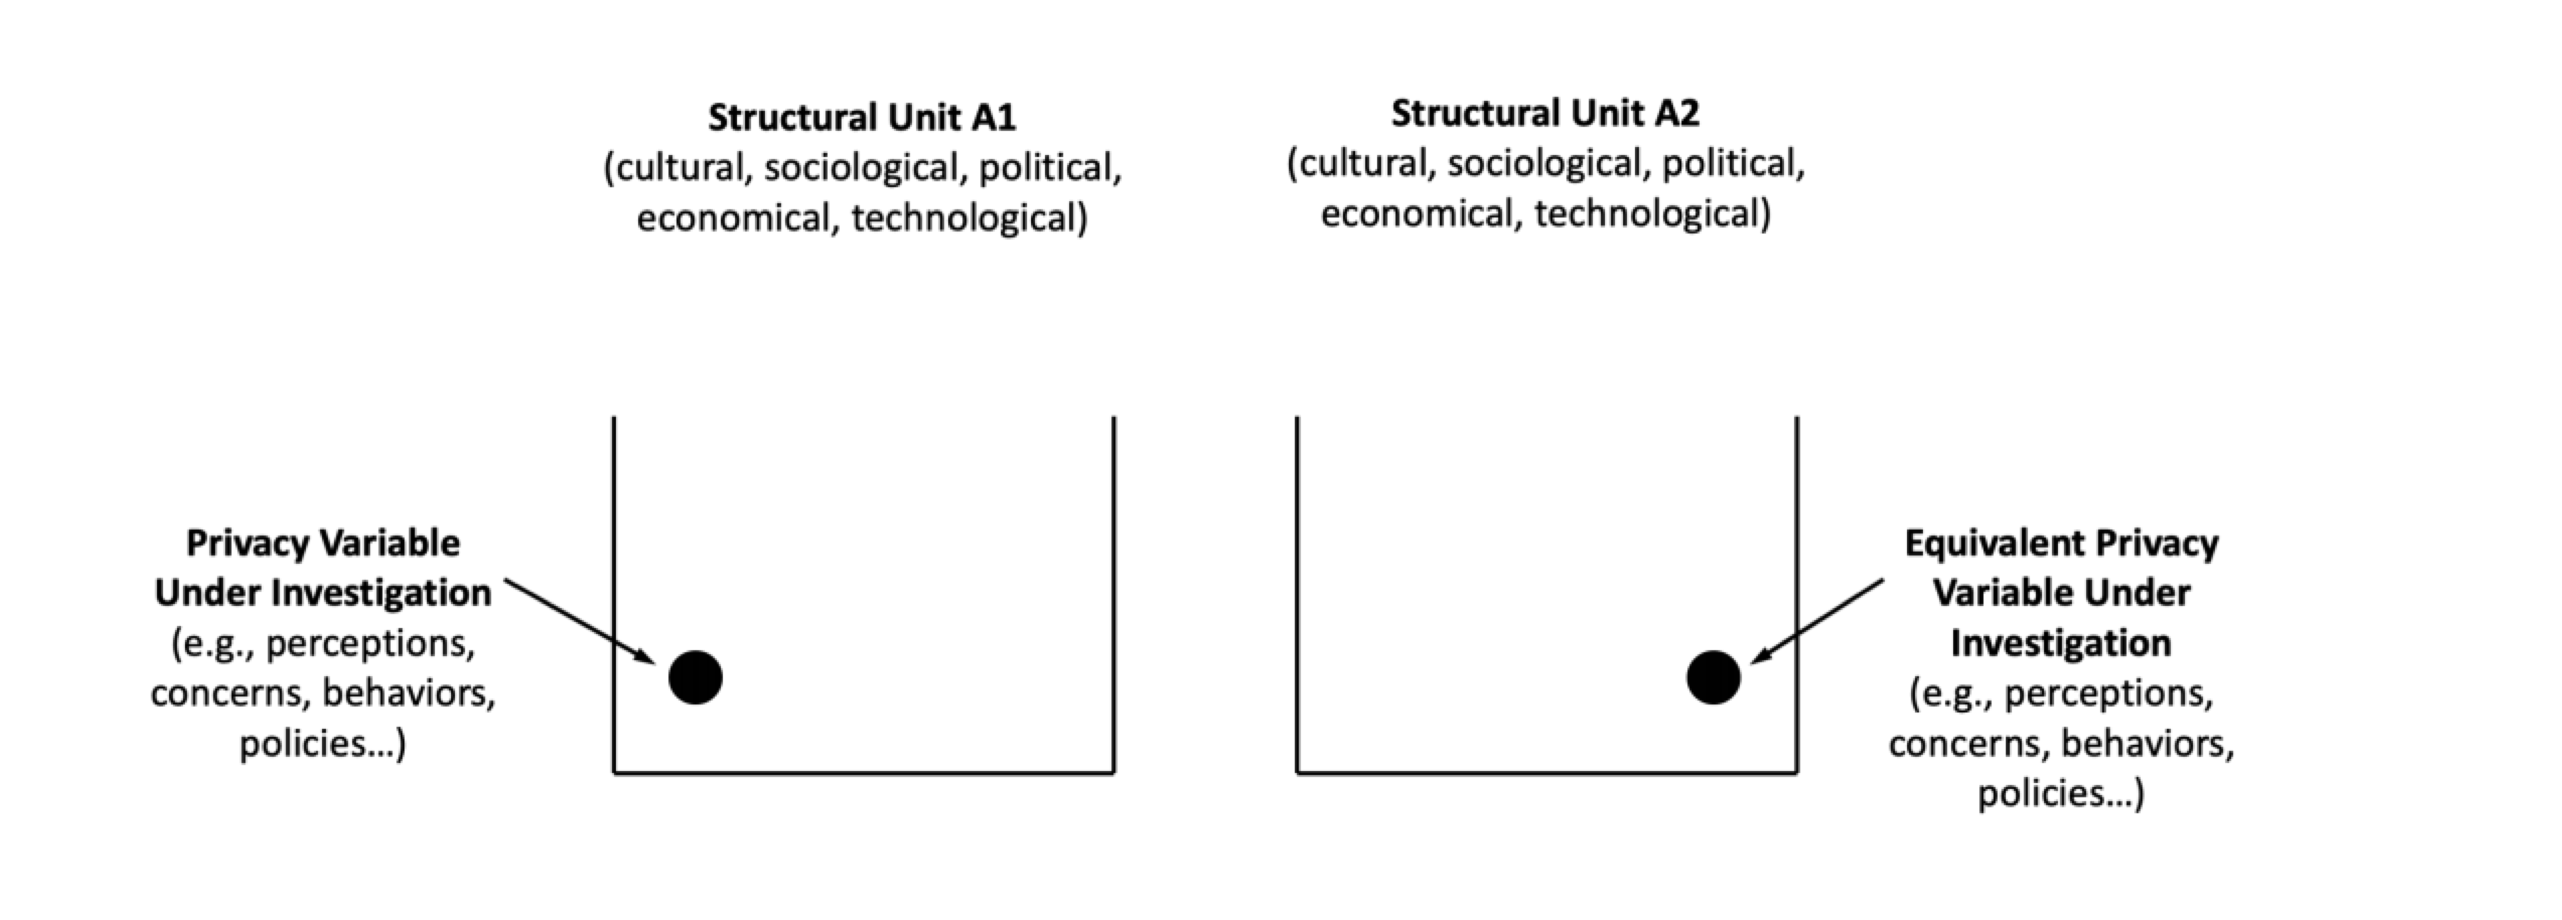
\includegraphics{img/entanglement.png}
\end{frame}

\begin{frame}{Comparative perspectives}
\protect\hypertarget{comparative-perspectives-1}{}
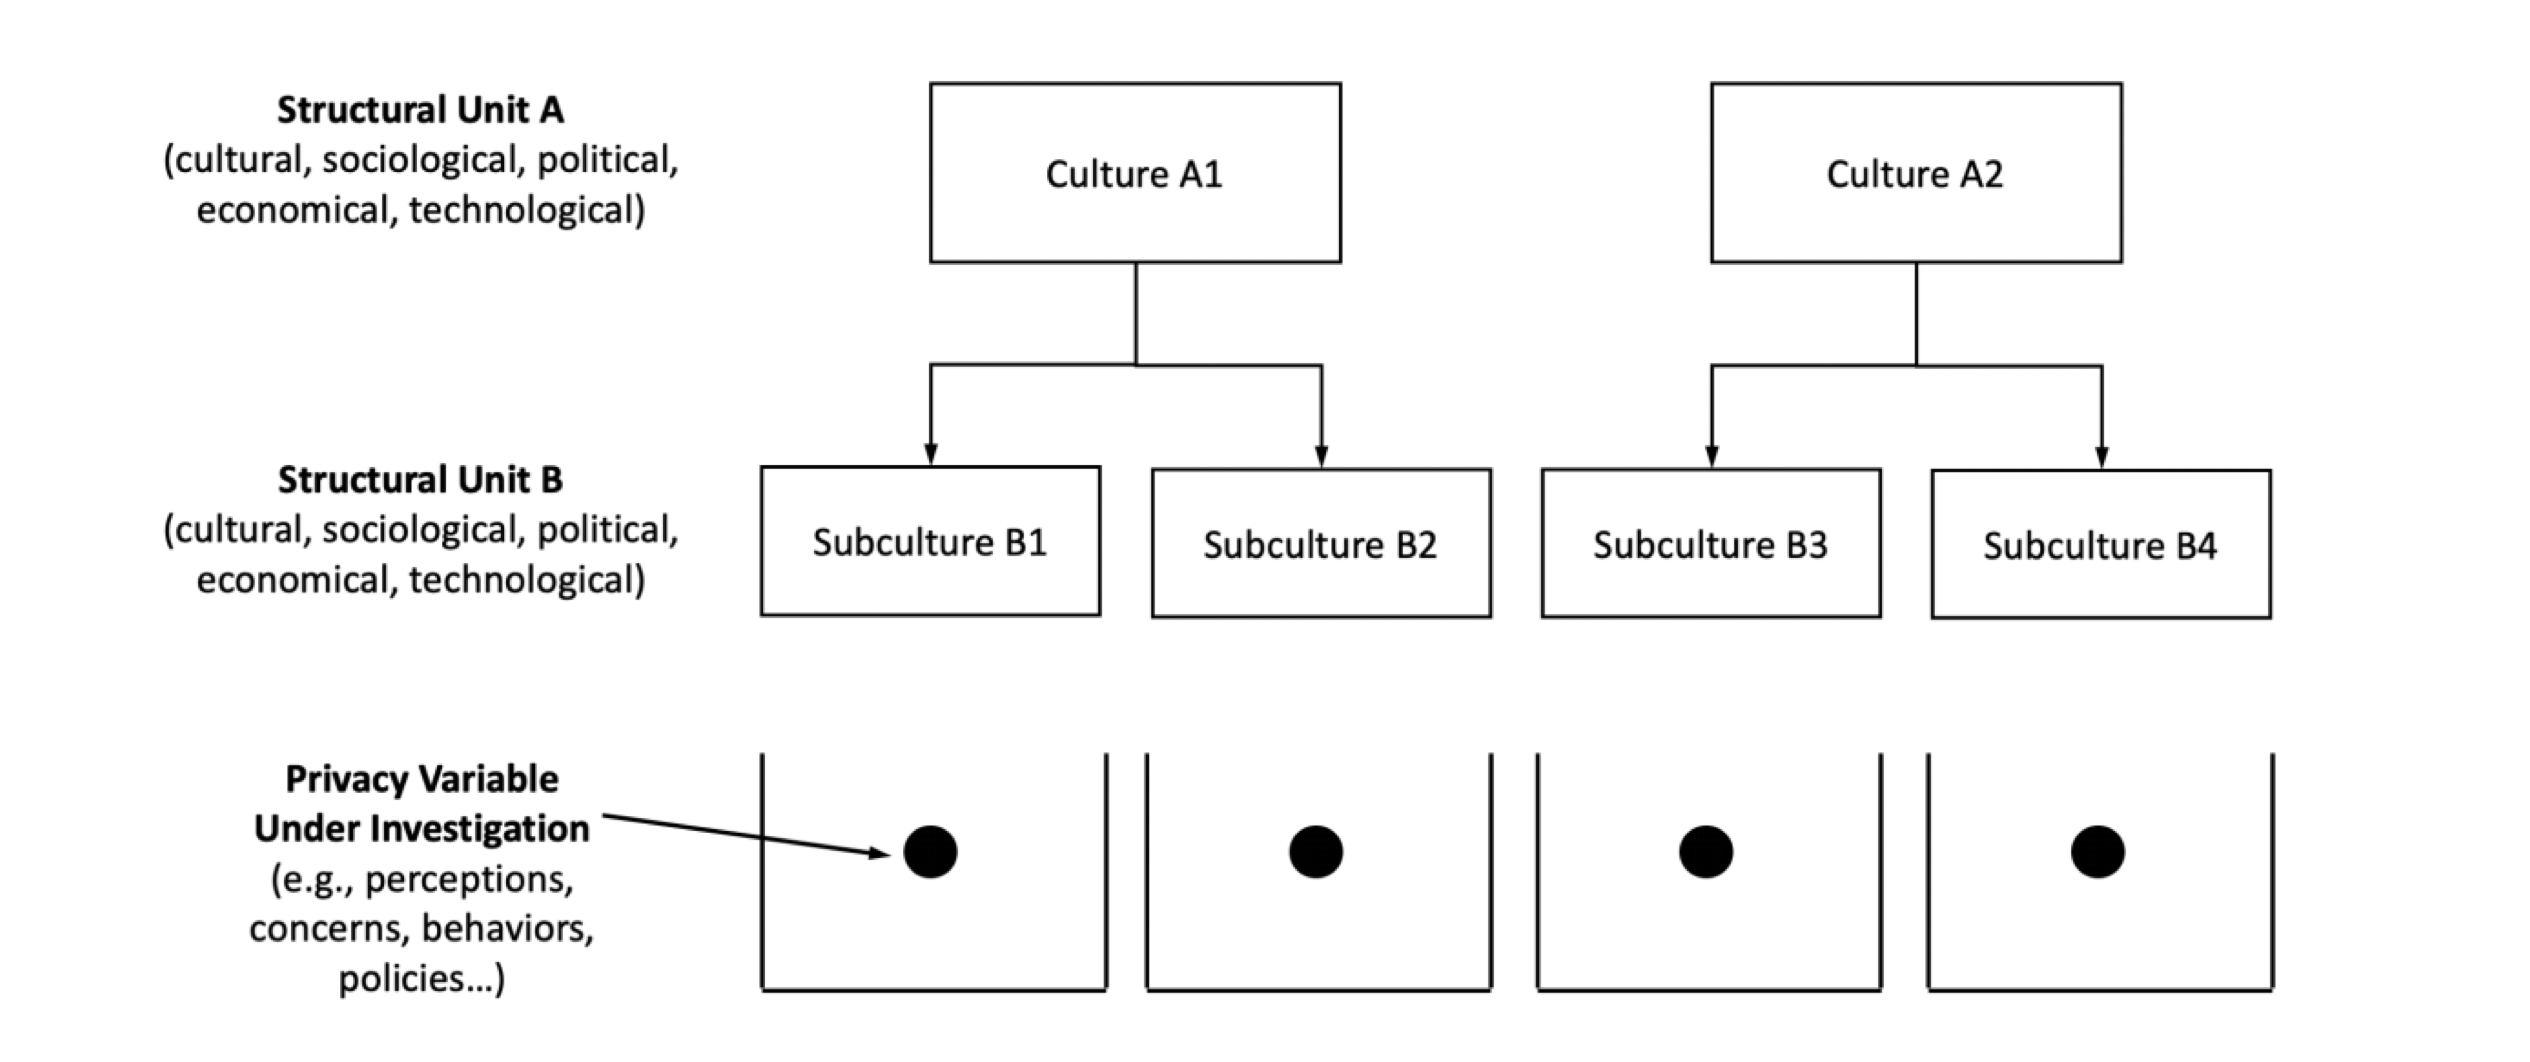
\includegraphics{img/entanglement2.png}
\end{frame}

\begin{frame}{Over the next two days\ldots{}}
\protect\hypertarget{over-the-next-two-days}{}
\ldots{} we want to learn more about:

\begin{enumerate}
\item
  ``specific cases'' (e.g., countries, platforms, groups\ldots)
\item
  existing comparative projects and perspectives
\item
  comparative methodologies and related challenges and innovations
\item
  most important research questions that could benefit from a
  comparative perspective
\end{enumerate}
\end{frame}

\begin{frame}{In the workshops\ldots{}}
\protect\hypertarget{in-the-workshops}{}
\ldots{} we are going to:

\begin{enumerate}
\item
  Generate ideas for comparative projects
\item
  Write first proposals
\item
  Pitch the ideas to the group
\item
  Hopefully provide inspiration for future collaboration
\end{enumerate}
\end{frame}

\hypertarget{thank-you-1}{%
\section{Thank you!}\label{thank-you-1}}



\end{document}
